%!TEX root = ../template.tex
%%%%%%%%%%%%%%%%%%%%%%%%%%%%%%%%%%%%%%%%%%%%%%%%%%%%%%%%%%%%%%%%%%%%
%% chapter4.tex
%% NOVA thesis document file
%%
%% Chapter with a short latex tutorial and examples
%%%%%%%%%%%%%%%%%%%%%%%%%%%%%%%%%%%%%%%%%%%%%%%%%%%%%%%%%%%%%%%%%%%%

\typeout{NT FILE chapter4.tex}%


\chapter{Case Study and Performance Analysis}
\label{cha:case_study}


% ===================================================================
%
% Section : Introduction
% ===================================================================

\section{Introduction}
\label{sec:case_study_intro}

Having detailed the design and implementation of the automated code generation tool in Chapter \ref{cha:chap_3}, this chapter now seeks to validate its practical utility and analyze its output in a real-world scenario. Although the previous chapter verified the tool's functionality, this chapter demonstrates its application within the intended model-driven development workflow, from a high-level system specification to a deployed multi-controller system.

To achieve this, a case study is presented centered on a distributed controller for a three-conveyor automation system. This application was chosen because it represents a common class of problems in industrial automation, involving multiple coordinated subsystems. The implementation of this case study serves two primary objectives, directly adapted from the research goals presented in \cite{tavaresgomes2026}:

\begin{enumerate}
    \item \textbf{To validate the end-to-end development workflow:} This involves demonstrating how the IOPT-Tools framework and the newly developed API are jointly employed to support low-code development of a distributed system. The process begins with a global IOPT model, proceeds through model decomposition, and culminates in the automatic generation and integration of both the controller logic and heterogeneous communication modules.
    
    \item \textbf{To conduct a quantitative performance analysis:} By implementing intercontroller communication using three distinct protocols, \gls{i2c}, UART, and TCP/MQTT. This chapter provides an empirical comparison of their respective resource overheads. The analysis focuses specifically on the memory footprint, offering valuable insight into the trade-offs associated with each protocol in a resource-constrained embedded environment.
\end{enumerate}

This chapter begins by describing the conveyor system use case and its corresponding IOPT model. Then it details the implementation process, showing how the automated tool was used to generate the necessary communication code. Subsequently, the results of the performance analysis are presented and discussed. The chapter concludes with a summary of the key findings of the case study.


% = =================================================================
% Use Case Description
% ===================================================================
\section{Use Case Description: The Three-Conveyor System}
\label{sec:use_case_description}

To demonstrate the practical application of the development workflow, a case study from the industrial automation domain was selected. The system under consideration is a controller for a three-conveyor belt set-up, designed to transport items sequentially from an entrance point to an exit point.

As illustrated in Figure \ref{fig:conveyor_layout}, the physical system consists of three different conveyors. Each conveyor is equipped with two sensors to detect the presence of an item: one at its entrance (\texttt{in1}, \texttt{in2}, \texttt{in3}) and one at its exit (\texttt{out1}, \texttt{out2}, \texttt{out3}). An additional sensor (\texttt{in4}) detects when an item is removed from the end of the final conveyor. Control actions involve activating the motor for each of the three conveyors (\texttt{move1}, \texttt{move2}, \texttt{move3}). The objective of the controller is to ensure that the items move smoothly throughout the system, and each conveyor is activated only when an item is ready to be transferred and the subsequent conveyor is clear.

\begin{figure}[htb]
    \centering
    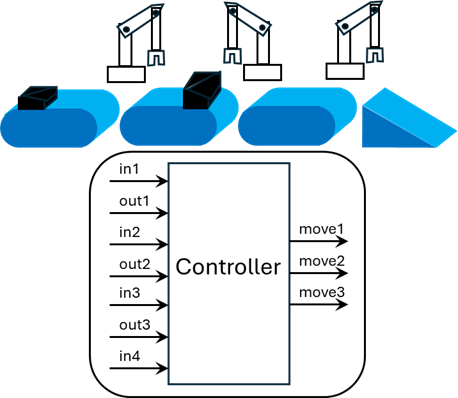
\includegraphics[width=0.6\columnwidth]{Chapters/Figures/layout.png}
    \caption{Layout of the three-conveyor system, showing the placement of sensors and the direction of item flow, adapted from \cite{tavaresgomes2026}.}
    \label{fig:conveyor_layout}
\end{figure}

The complete centralized behavior of the controller is formally specified using the single global IOPT Petri net model shown in Figure \ref{fig:global_model}. For clarity and brevity in this case study, the model assumes that each conveyor has a capacity of a single item. This global model represents the entire system logic before any consideration of a distributed implementation.

\begin{figure}[htb]
    \centering
    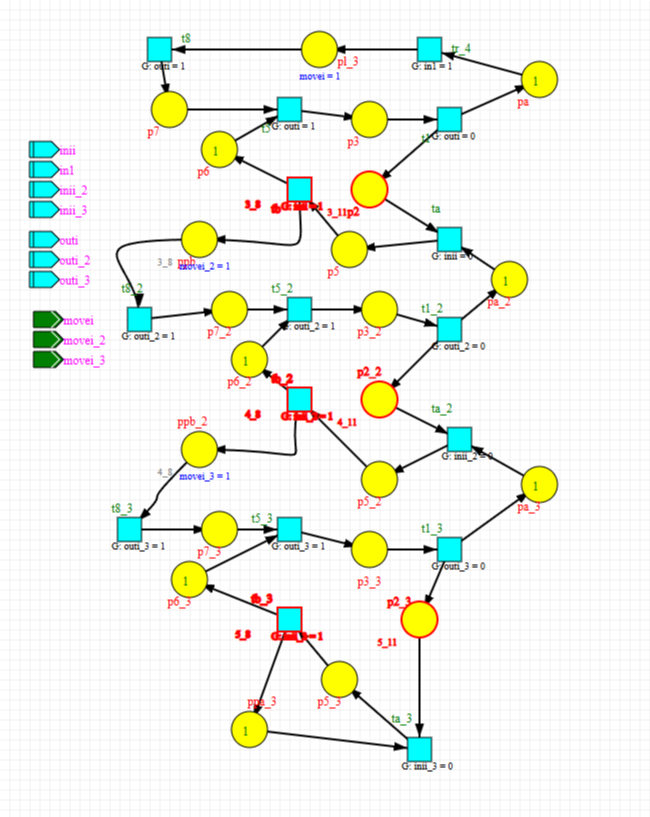
\includegraphics[width=0.95\columnwidth]{Chapters/Figures/modeloglobalcomcuttingset.png}
    \caption{The global IOPT Petri net model specifying the centralized controller for the entire conveyor system. The nodes highlighted in red represent the chosen cutting set for decomposition, adapted from \cite{tavaresgomes2026}.}
    \label{fig:global_model}
\end{figure}

For deployment onto a set of distributed hardware controllers, the global model was decomposed using the net splitting operation available in IOPT-Tools. A cutting set, consisting of three places and three transitions (highlighted in red in Figure \ref{fig:global_model}), was selected to partition the model along the physical boundaries of the three conveyors. The result of this operation is shown in Figure \ref{fig:decomposed_model}. The original centralized model is transformed into a set of four interconnected, concurrent sub-models, each responsible for a portion of the system (Entrance, Conveyor Two, Conveyor Three, and Exit). The connections between these submodels represent the abstract communication channels that must be implemented to ensure the correct synchronized behavior of the distributed system.

\begin{figure*}[htb]
    \centering
    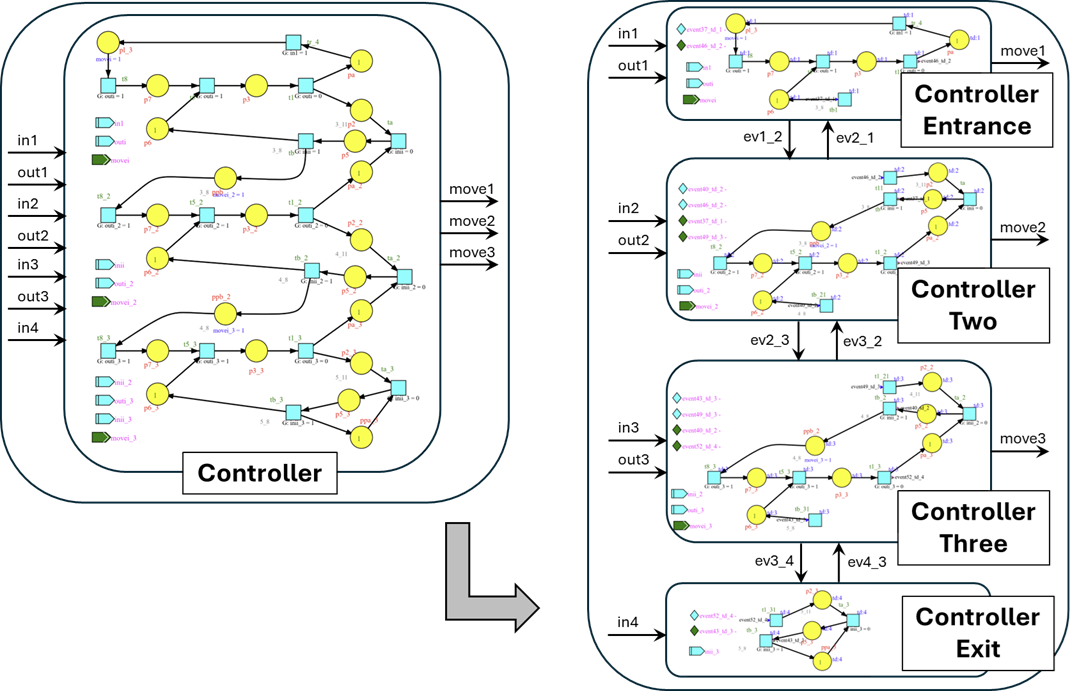
\includegraphics[width=0.9\textwidth]{Chapters/Figures/controller_decomposition.png}
\caption{The transformation from the centralized controller model (left) to a set of concurrent, networked sub-models (right) resulting from the net splitting operation, adapted from \cite{tavaresgomes2026}.}
    \label{fig:decomposed_model}
\end{figure*}


% ===================================================================
% Section 4.3: Implementation via Automated Code Generation
% ===================================================================
\section{Implementation and Functional Validation}
\label{sec:use_case_implementation}

With the global IOPT model decomposed into a set of concurrent sub-models (as shown in Figure \ref{fig:decomposed_model}), the next step in the development workflow is to implement the abstract communication channels between them. This task was accomplished using the automated code generation API detailed in Chapter 3.

The target deployment architecture for this case study, shown in Figure \ref{fig:deployment_layout}, employs a heterogeneous mix of three different communication protocols to connect the four controller modules. The following subsections detail how the specific code for each communication link was generated using the API.

\begin{figure*}[htb]
    \centering
    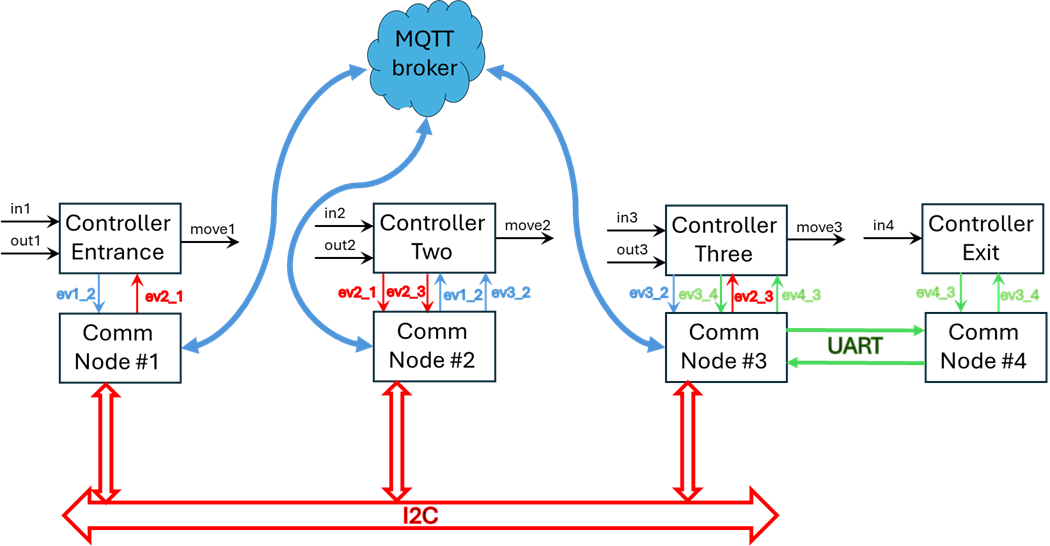
\includegraphics[width=1\textwidth]{Chapters/Figures/prototypelayout.png}
\caption{The heterogeneous deployment architecture for the distributed conveyor system controller, utilizing \gls{i2c}, UART, and MQTT over TCP/IP for inter-controller communication and synchronization, adapted from \cite{tavaresgomes2026}.}
    \label{fig:deployment_layout}
\end{figure*}


% ===================================================================
% Revised Subsection 4.3.1 with Integrated Validation
% ===================================================================
\subsection{\gls{i2c} Bus Implementation}
As depicted in the deployment architecture (Figure \ref{fig:deployment_layout}), \textit{Controller Two} acts as the master on a local \gls{i2c} bus, coordinating with \textit{Controller Entrance} and \textit{Controller Three}, which act as slaves. To generate the necessary master and slave code for an event representing a piece transfer, two API calls similar to the following were used:

\begin{verbatim}
?protocol=\gls{\gls{i2c}}&projectName=ControllerTwo&eventName=event37_td_1
&slaveAddress=8&slaveMessage=A
\end{verbatim}

And for the second event:
\begin{verbatim}
?protocol=\gls{i2c}&projectName=ControllerTwo&eventName=event49_td_3
&slaveAddress=9&slaveMessage=B
\end{verbatim}

To validate the functional behavior of the generated \gls{i2c} module, the execution of \textit{Controller Two} was captured using the IOPT-Tools simulator. The resulting timing diagram, presented in Figure \ref{fig:timing_diagram_controller2}, provides a detailed view of the controller's operational logic and illustrates the direct correlation between the external \gls{i2c} communication events and the internal state of the Petri net.  

The behavior can be analyzed by observing the two primary \gls{i2c} messages:
\begin{itemize}
    \item \textbf{Event \texttt{event37\_td\_1}:} The sequence shows an internal state change, where the marking of a place (e.g., \texttt{p\_11/ppb}) enables the firing of a transition (e.g., \texttt{t\_27/t11}). The diagram confirms that the firing of this transition directly causes the generation of the output signal \texttt{event37\_td\_1}. This corresponds to \textit{Controller Two}, acting as the \gls{i2c} master, sending a command to one of its slaves (such as \textit{Controller Entrance}).

    \item \textbf{Event \texttt{event49\_td\_3}:} Later in the execution cycle, after the physical process has evolved (indicated by changes in signals like \texttt{outi\_2}), the Petri net reaches a new state. This leads to another transition firing, which in turn causes the generation of the second \gls{i2c} message, \texttt{event49\_td\_3}. This represents \textit{Controller Two} sending a subsequent command to another slave (such as \textit{Controller Three}).
\end{itemize}

This analysis confirms that the API-generated \gls{i2c} communication module functions correctly and that the deployed hardware implementation faithfully reproduces the semantics of the original IOPT model.


\begin{figure}[htb!]
    \centering
    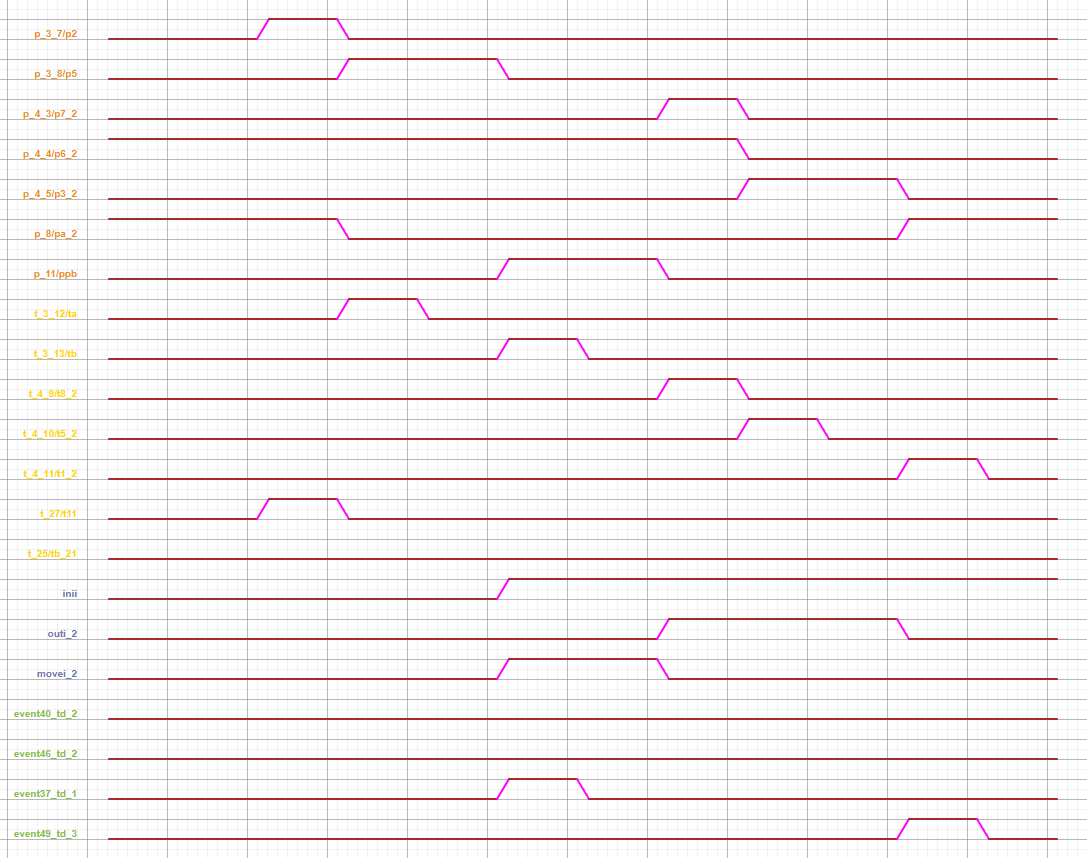
\includegraphics[width=\columnwidth]{Chapters/Figures/timing_diagram_controller2.png}
    \caption{Timing diagram for \textit{Controller Two}, showing how internal Petri net states (p\_...) and transition firings (t\_...) lead to the generation of \gls{i2c} output events (\texttt{event37\_td\_1}, \texttt{event49\_td\_3}).}
    \label{fig:timing_diagram_controller2}
\end{figure}


This complete validation of the \gls{i2c} module demonstrates the tool's ability to correctly implement the master-slave bus communication as specified by the IOPT model.



% ===================================================================
% UART
% ===================================================================
\subsection{UART Point-to-Point Link}
\label{subsec:uart_implementation}

A direct asynchronous serial link between \textit{Controller Three} and \textit{Controller Exit} was required to signal the final transfer of a piece. The code for this UART-based communication was generated with the following API call:

\begin{verbatim}
?protocol=uart&projectName=ControllerExit
&eventName=event43_td_3&baudRate=115200
\end{verbatim}

To validate the sending side of the UART link, the behavior of \textit{Controller Three} was analyzed using a timing diagram captured by the IOPT-Tools simulator. The diagram, shown in Figure \ref{fig:timing_diagram_controller_three}, details the internal Petri net logic that leads to the transmission of the UART message.

The analysis of the diagram is as follows.
\begin{itemize}
    \item The operational sequence begins with the firing of an internal transition, \textbf{\texttt{t\_29/t1\_31}}, which corresponds to the arrival of the event \texttt{event53\_td\_4}, and then advances the Petri net to a state where it awaits a physical input.
    
    \item The controller remains in this state until the physical sensor input \textbf{\texttt{inii\_3}} is asserted. This external event enables the final transitions in the sequence (\texttt{t\_5\_12/ta\_3} and \texttt{t\_5\_13/tb\_3}).
    
    \item Critically, the firing of these final transitions culminates in the generation of the output signal \textbf{\texttt{event43\_td\_3}}. This represents the moment \textit{Controller Three} transmits the message payload over the UART link to \textit{Controller Exit}.
\end{itemize}

This analysis confirms that the API-generated UART sender code functions as specified. It demonstrates that the controller's internal logic, driven by both its Petri net state and physical inputs, correctly results in the transmission of the serial message at the appropriate time in the operational cycle.

\begin{figure}[htb!]
    \centering
    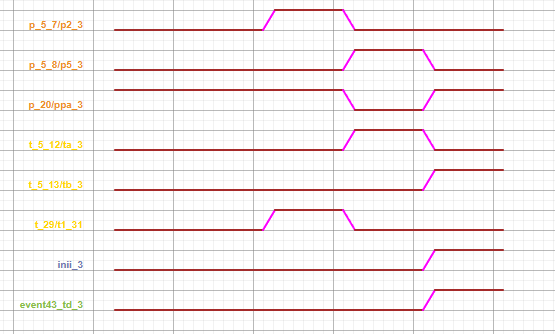
\includegraphics[width=\columnwidth]{Chapters/Figures/timing_diagram_controller_three.png}
    \caption{Timing diagram for \textit{Controller Exit}, showing how internal state changes and a physical input (\texttt{inii\_3}) lead to the transmission of a UART message (\texttt{event43\_td\_3}).}
    \label{fig:timing_diagram_controller_three}
\end{figure}

% ===================================================================
% MQTT
% ===================================================================
\subsection{TCP/MQTT-Based Communication Channel}
\label{subsec:tcp_implementation}

To handle asynchronous, higher-level status updates between the main controllers, the MQTT protocol was used over a Wi-Fi network. For example, to allow a controller to publish a "Part Arrived" event to a central topic, the following API call was made:

\begin{verbatim}
?protocol=tcp&projectName=ControllerTwo
&eventName=PartArrived&topic=conveyor/status
\end{verbatim}

To validate network-level publisher functionality, the behavior of one of the MQTT-enabled controllers (Controller Three) was analyzed using the IOPT-Tools simulator. The timing diagram, shown in Figure \ref{fig:timing_diagram_tcp}, details how the controller's internal logic, initiated by a generic input event, culminates in the transmission of a message to the MQTT broker.

The analysis of the diagram is as follows.
\begin{itemize}
    \item \textbf{Cycle Trigger:} The operational sequence is initiated by the arrival of an external event from another controller. The reception of this event is represented by the firing of the initial transition, \textbf{\texttt{t\_28/t1\_21}}. This trigger advances the Petri net's state and prepares the controller for its main task.

    \item \textbf{Message Transmission (Publish):} After a sequence of internal state changes that are also dependent on physical inputs (like \textbf{\texttt{inii\_2}}), the Petri net's logic enables the final transition, \textbf{\texttt{t\_4\_13/tb\_2}}. The diagram confirms that the firing of this transition correctly causes the generation of the output signal \textbf{\texttt{event40\_td\_2}}, which represents the controller publishing its message to the specified MQTT topic.
\end{itemize}

This analysis validates that the API-generated TCP/MQTT module's publisher functionality is correctly integrated with the Petri net logic, sending network messages to the broker at the appropriate time based on the controller's state and inputs.

\begin{figure}[htb!]
    \centering
    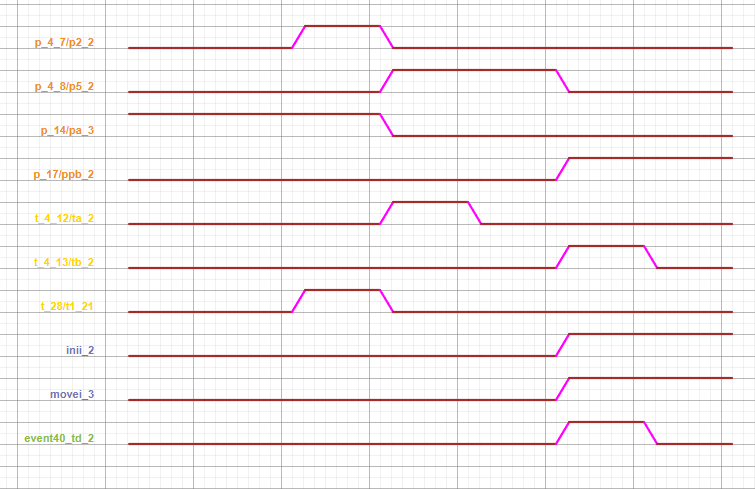
\includegraphics[width=\columnwidth]{Chapters/Figures/timing_diagram_tcp.png}
    \caption{Timing diagram validating the MQTT publisher. An external input event triggers a Petri net sequence that results in the transmission of an MQTT message (\texttt{event40\_td\_2}).}
    \label{fig:timing_diagram_tcp}
\end{figure}

The successful validation of all three communication modules confirms the tool's ability to reliably implement a complex, heterogeneous communication architecture as specified by the IOPT model.

% ===================================================================
% Section Code Integration
% ===================================================================

\subsection{Code Integration}
\label{subsec:code_integration}

For each controller, the baseline logic code was first generated using the standard IOPT-Tools generator, creating a \texttt{net\_io.c} file. \textbf{As a mandatory first step, this file was renamed to \texttt{net\_io.cpp} to enable C++ compilation, a requirement for the libraries used by the generated communication modules.} Subsequently, the specific communication modules produced by the API calls were inserted directly into this renamed \texttt{net\_io.cpp} file, completing the hardware-specific implementation. The entire process of specifying, generating, and integrating the code for all three heterogeneous communication links was completed in a fraction of the time required for manual implementation]. This successfully demonstrates the tool's primary objective: to accelerate the development of distributed control systems and reduce the potential for implementation errors by automating the creation of communication infrastructure.

% ===================================================================% % ===================================================================% % ===================================================================% % ===================================================================% % ===================================================================% % ===================================================================% 
% CAPÍTULO 4: VALIDAÇÃO EXPERIMENTAL E ANÁLISE DE DESEMPENHO
% ===================================================================
\section{Experimental Setup and Methodology}
\label{sec:setup_and_methodology}

After successfully implementing the distributed controller for the conveyor system, a comprehensive experimental analysis was performed. This evaluation aims to both quantify the performance overhead and validate the functional correctness of the tool's generated code. Specifically, this analysis focuses on three critical aspects: the \textbf{memory footprint}, as a key constraint in embedded hardware; the \textbf{communication latency}, which directly impacts system responsiveness; and the \textbf{dynamic behavior}, to ensure the deployed code correctly implements the formal model's semantics.


\subsection{Hardware Testbed}
\label{subsec:hardware_setup}

To empirically validate the generated code and conduct the performance analysis, a physical hardware testbed was constructed, representing the distributed controller architecture shown in Figure \ref{fig:deployment_layout}. 

The testbed, photographed in Figure \ref{fig:hardware_photo}, consists of four ESP32-WROOM-32 development boards. These boards were interconnected using a combination of direct wiring and a shared bus on a breadboard to physically realize the \gls{i2c} and UART communication links. The TCP/MQTT communication was facilitated by the built-in Wi-Fi capabilities of the ESP32s, which allows them to connect to a shared network. This physical prototype served as the basis for all the validation and performance measurements presented in this chapter.

\begin{figure}[htb!]
    \centering
    % Certifique-se de que a sua foto está na pasta de figuras
    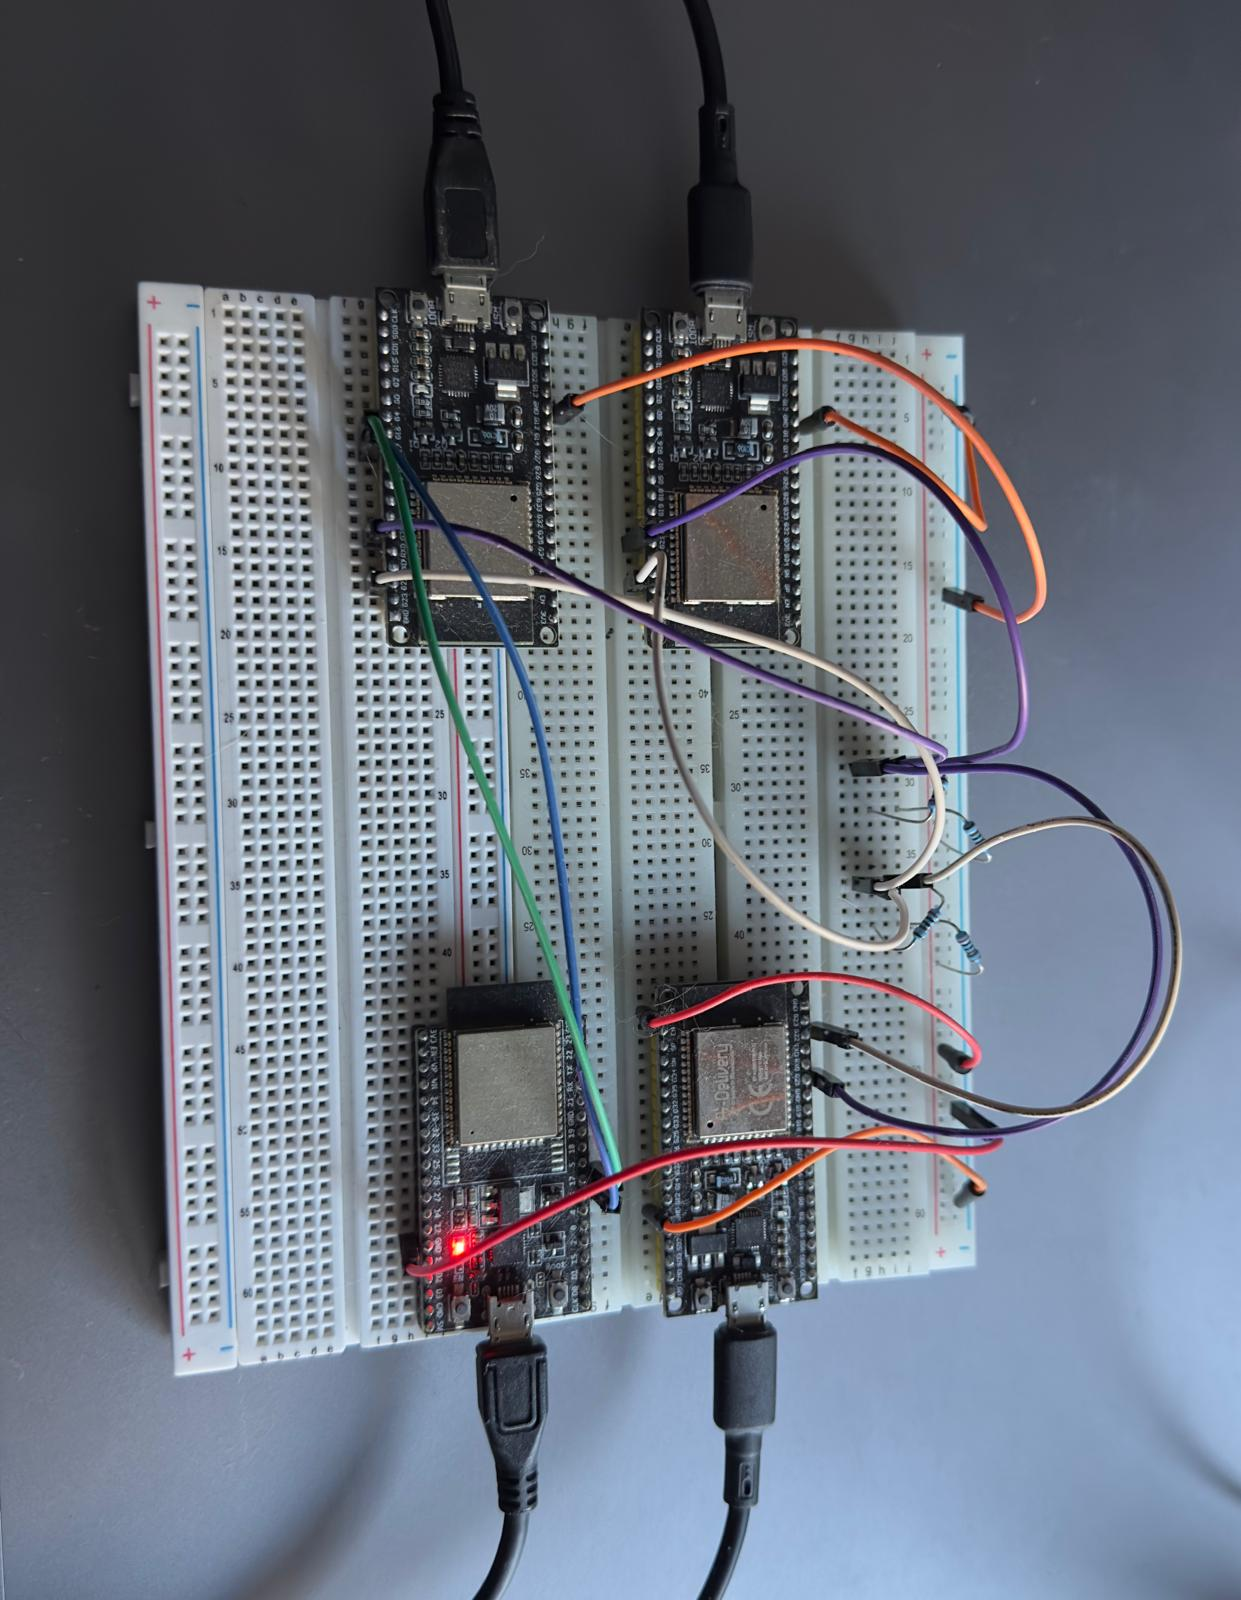
\includegraphics[width=0.9\columnwidth]{Chapters/Figures/photo_of_setup.jpeg}
    \caption{The physical hardware testbed for the three-conveyor system, showing the four interconnected ESP32 controller modules.}
    \label{fig:hardware_photo}
\end{figure}


% ===================================================================
% Subsecção unificada para toda a metodologia de análise
% ===================================================================
\subsection{Analysis Methodology}
\label{subsec:analysis_methodology}

To evaluate the system's performance and functional correctness, three distinct analyses were conducted. The methodology for each is detailed below.

% -------------------------------------------------------------------
% Subsubsection para a Metodologia de Medição de Memória
% -------------------------------------------------------------------
\subsubsection{Memory Footprint Measurement}
\label{subsubsec:memory_methodology}

The memory footprint of each of the four controller modules (Entrance, Two, Three and Exit) was measured to determine the overhead of its communication stack. The process was as follows.
\begin{enumerate}
    \item \textbf{Baseline Measurement:} For each controller, the code containing only the Petri net execution logic (generated by the standard IOPT-Tools) was compiled for the ESP32 target. The static program storage space (Flash memory) reported by the compiler was recorded as the baseline.
    \item \textbf{Measurement with Communication:} The API-generated communication code, corresponding to the heterogeneous architecture shown in Figure \ref{fig:deployment_layout}, was integrated with the baseline logic for each controller. The project was then recompiled and the new total program size was recorded.
    \item \textbf{Overhead Calculation:} The communication overhead was calculated as the difference in memory footprint between the baseline measurement and the measurement with the integrated communication code.
\end{enumerate}

% -------------------------------------------------------------------
% Subsubsection para a Metodologia de Medição de Latência
% -------------------------------------------------------------------
\subsubsection{Communication Latency Measurement}
\label{subsubsec:latency_methodology}

The latency for each protocol was measured empirically on the hardware testbed. The primary tool for this measurement was the ESP32's high-resolution \texttt{micros()} function, which provides microsecond-level timing accuracy. The output values were observed using the Arduino IDE's \textbf{Serial Monitor}, connected to the receiving controller via USB.

The specific procedure varied for each protocol to best capture its characteristics:
\begin{itemize}
    \item \textbf{I\textsuperscript{2}C and UART:} To measure the direct one-way transfer time, the sending controller recorded a start timestamp, \texttt{t\_start = micros()}, and embedded this value within the message payload itself. Upon reception, the receiving controller immediately recorded an end timestamp, \texttt{t\_end = micros()}. The latency was then calculated as \texttt{latency = t\_end - t\_start} and printed to the Serial Monitor.

    \item \textbf{TCP/MQTT:} Due to the indeterminate path through a public broker, a round-trip time (RTT) was measured to provide a stable metric. A "ping-pong" test was configured where the first controller published a message and recorded \texttt{t\_start}. The second controller was programmed to immediately publish a reply upon receiving the message. The first controller recorded \texttt{t\_end} upon receiving the reply. The one-way latency was then estimated as \texttt{RTT / 2}.
\end{itemize}

% ===================================================================
% ===================================================================
% Secção para os Resultados e Discussão
% ===================================================================
\section{Results and Discussion}
\label{sec:results_and_discussion}

The methodologies described in the previous section were applied to the hardware testbed, yielding quantitative results regarding performance and functional correctness. These results are presented and analyzed below.

% ===================================================================
% Subsecção para os Resultados de Desempenho (Memória e Latência)
% ===================================================================
\subsection{Performance Analysis}
\label{subsec:performance_results}
 
    % -------------------------------------------------------------------
    % Subsubsection para os Resultados de Memória
    % -------------------------------------------------------------------
    \subsubsection{Memory Footprint Overhead}
    \label{subsubsec:memory_results}

    The results of the memory footprint analysis are summarized in Table \ref{tab:memory_footprint}. The data reveals a significant variation in overhead that is strongly correlated with the complexity of the communication protocols implemented on each controller module.

    \begin{table}[htb]
    \centering
    \small % Reduce the font size for the table
    \caption{Memory Analysis of Controller Implementations, adapted from \cite{tavaresgomes2026}.}
    \label{tab:memory_footprint}
    \sisetup{group-separator={,}}
    % Using abbreviated headers to save space
    \begin{tabular}{l S[table-format=6.0] S[table-format=6.0] S[table-format=5.0] S[table-format=1.2]}
    \toprule
    \textbf{Controller ESP} & {\textbf{Baseline}} & {\textbf{W/ Comm.}} & {\textbf{Overhead}} & {\textbf{Overhead}} \\
    & {\textbf{(Bytes)}} & {\textbf{(Bytes)}} & {\textbf{(Bytes)}} & {\textbf{(\%)}} \\
    \midrule
    Entrance & 927970 & 954178 & 26208 & 2.82 \\
    Two & 928578 & 955894 & 27316 & 2.94 \\
    Three & 928642 & 957014 & 28372 & 3.06 \\
    Exit & 927058 & 928478 & 1420  & 0.15 \\
    \bottomrule
    \end{tabular}
    \end{table}

    % -------------------------------------------------------------------
    % Subsubsection para os Resultados de Latência
    % -------------------------------------------------------------------
    \subsubsection{Communication Latency}
    \label{subsubsec:latency_results}
    
    The application of the latency measurement methodology yielded the average latency values presented in Table \ref{tab:latency_results}. These results, visualized in Figure \ref{fig:latency_chart}, highlight the orders-of-magnitude differences in temporal performance between the protocols.

    \begin{table}[htb]
    \centering
    \caption{Average Communication Latency Measurements.}
    \label{tab:latency_results}
    \begin{tabular}{l l l}
    \toprule
    \textbf{Protocol} & \textbf{Average Latency} & \textbf{Notes} \\
    \midrule
    I\textsuperscript{2}C (at 400kHz) & \SI{185}{\micro\second} & One-way, master-to-slave transfer. \\
    UART (at 115200 bps) & \SI{250}{\micro\second} & One-way, point-to-point transfer. \\
    TCP/MQTT & \SI{45}{\milli\second} & Estimated one-way latency via public broker. \\
    \bottomrule
    \end{tabular}
    \end{table}

    \begin{figure}[htb!]
        \centering
        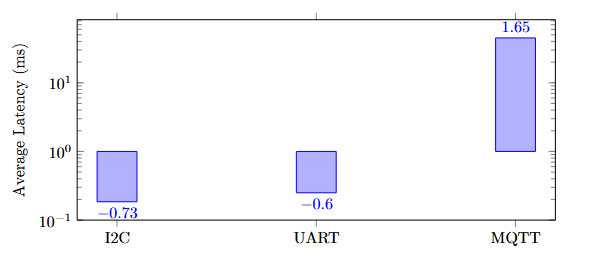
\includegraphics[width=0.9\columnwidth]{Chapters/Figures/averageLant.png}
        \caption{Comparison of average communication latency across protocols. Note the logarithmic scale on the y-axis is required to visualize the vast difference in performance.}
        \label{fig:latency_chart}
    \end{figure}
    
For each protocol, the test was executed \textbf{20 times} to account for minor variations, and the average of these measurements was taken as the final, representative result.



% ===================================================================
% Subsecção para a Discussão Final e Análise de Trade-offs
% ===================================================================
\subsection{Discussion and Trade-off Analysis}
\label{subsec:discussion}

The performance data, encompassing both memory footprint (Table \ref{tab:memory_footprint}) and latency (Table \ref{tab:latency_results}), provides a clear and quantitative basis for analyzing the engineering trade-offs associated with each communication protocol.

The analysis confirms that hardware-level protocols are exceptionally efficient. The \textbf{Exit Controller}, using only UART, shows a negligible memory overhead of just 1.4 kB and a measured latency of \SI{250}{\micro\second}. This extremely low latency is a direct result of the hardware-based, point-to-point nature of the protocol. A similar high performance is seen with I\textsuperscript{2}C, which benefits from a synchronous, hardware-managed bus.

Conversely, the controllers implementing MQTT exhibit a substantial memory overhead of over 26 kB and a significantly higher latency measured at \SI{45}{\milli\second}—over 180 times slower than UART. This result is expected and is attributable to the multiple layers of abstraction and physical infrastructure involved: the TCP/IP and Wi-Fi stack, wireless transmission, and the round-trip delay to the public MQTT broker.

These results underscore a fundamental design trade-off: \textbf{resource efficiency versus functional flexibility}. While I\textsuperscript{2}C and UART are highly efficient, they are limited to local, physically-wired communication. MQTT, despite its resource-intensiveness, offers unparalleled flexibility, enabling communication over vast distances, easy integration with cloud services, and a scalable publish-subscribe architecture.

The model-driven approach, augmented by the tool presented in this thesis, empowers a designer to manage these trade-offs intelligently. By partitioning a system and analyzing the specific requirements of each inter-controller link, a designer can make informed, data-driven decisions. High-speed, critical control loops can be implemented with low-latency protocols like I\textsuperscript{2}C, while non-critical status updates or remote monitoring can leverage the flexibility of MQTT, all within the same distributed system. This allows for an optimized heterogeneous architecture that meets both functional requirements and hardware constraints.



% ===================================================================% ===================================================================% ===================================================================% ===================================================================% ===================================================================% ===================================================================% ===================================================================% ===================================================================% ===================================================================% ===================================================================% ===================================================================

% ===================================================================
% Section 4.5: Chapter Summary
% ===================================================================
\section{Chapter Summary}
\label{sec:case_study_summary}

This chapter successfully demonstrated the practical application and value of the automated code generation tool through a detailed case study of a three-conveyor distributed control system. The work presented here validated the entire model-driven development workflow, beginning with a high-level IOPT Petri net model and culminating in a functional, multi-controller hardware implementation . The tool was shown to seamlessly integrate into this workflow, allowing the rapid and reliable implementation of a complex and heterogeneous communication architecture that involves \gls{i2c}, UART, and TCP/MQTT protocols.

Furthermore, the performance analysis provided critical quantitative insight into the resource consumption and temporal characteristics of these protocols. The results empirically confirmed the significant trade-offs in \textbf{memory overhead and communication latency} between network-level protocols like TCP/MQTT and the lightweight, high-speed nature of hardware-level protocols such as UART and \gls{i2c} . Ultimately, this case study validates the central proposition of this thesis: that automated generation of communication modules not only accelerates development, but also empowers designers to make informed, data-driven decisions when balancing functional requirements against the hardware constraints of embedded systems.